\chapter{Обзор предметной области}
Оптическое волокно — нить из оптически прозрачного материала (стекло, пластик), используемая для переноса света внутри себя посредством полного внутреннего отражения. Для объяснения этого явления рассмотрим процессы происходящие при прохожении светом границы двух сред:

При переходе в другую среду свети отклоняется от направления своего распространения. Величина этого отклонения определяется законом Снеллиуса:

\begin{equation}
 n_1 \sin\theta_1 = n_2 \sin\theta_2
\end{equation}

\begin{figure}[h!]
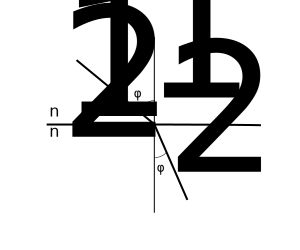
\includegraphics[width=0.5\textwidth]{img/refraction.pdf}
\caption{Преломление света}
\end{figure}

Очевидно, что при некотором угле падения синус соответствуюшего угла преломленния окажется больше единицы, что невозможно. В этом случае будет наблюдаться эффект полного внутреннего отражения. Это возможно только в случае $n_1 > n_2$

\begin{figure}[h!]
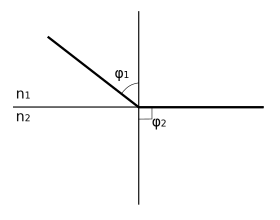
\includegraphics[width=0.5\textwidth]{img/refraction_full_inner.pdf}
\caption{Полное внутреннее отражение}
\end{figure}

\section{Планарные волноводы}
Планарный волновод - это структура из слоев с тремя разными показателями преломления с соотношением $n_f > n_s > n_c$ Свет, попадая в волновод, испытывает ПВО последовательно от обеих границ и оказывается заключен в волноводной среде и рапространяется вдоль нее с максимальной эффективностью

\begin{figure}[h!]
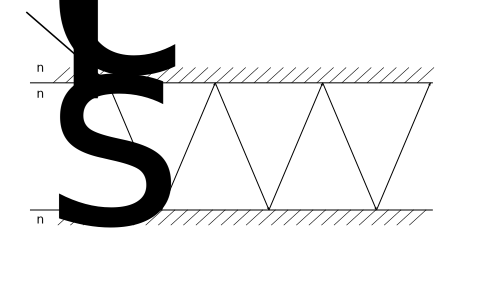
\includegraphics[width=0.9\textwidth]{img/planar_propagation.pdf}
\caption{Распространение света в волноводе}
\end{figure}

\section{Цилиндрические волноводы}
Наряду с волноводами прямоугольного сечения применяются также цилиндрические волноводы круглого сечения. Как правило, такие волноводы состоят из сердцевины и с высоким показателем преломления и оболочки, с меньшим показателем преломления. Для нахожения распределения поля в волноводе необходимо решить характеристическое уравнение, основанное вычислении набега фазы на пути луча отрезке AB двумя способами:
\begin{enumerate} 
	\item Путем сложения набегов фазы, обусловленных длиной тректории и отраженисм от стенок 
	\item Путем определения угла поворота $\Delta \phi$ и сдвига $\Delta z$ траектории луча на отрезке AB. В этом случае набег фазы находится как сумма:
	\begin{enumerate} 
		\item $\Delta z$ умноженного на продольную компоненту волнового вектора
		\item угла поворота, умноженного на тангенциальную компоненту волнового вектора, на радиус сердцевины $a$ волокна
	\end{enumerate}
\end{enumerate}

Конечное характеристическое уравнение примет такой вид \cite{adams}: